\documentclass[a4paper,12pt,titlepage,oneside]{book}
\pdfpagewidth
\paperwidth
\pdfpageheight
\paperheight
\pagestyle{plain}
\usepackage[main = italian, english]{babel}
\usepackage{amsmath,amssymb}
\usepackage{lmodern}
\usepackage[T1]{fontenc}
\usepackage[utf8]{inputenc}
\usepackage[usenames,dvipsnames]{xcolor}
\usepackage{graphicx,color,listings}
\frenchspacing
\usepackage{geometry}
\usepackage{rotating}
\usepackage{caption}
\usepackage{multirow}
\usepackage{hyperref}
\usepackage{graphicx}
\hypersetup{
    colorlinks=true,
    linkcolor=black,
    filecolor=blue,      
    urlcolor=blue,
    pdftitle={Documentazione Macchina Di Turing Universale},
    pdfpagemode=FullScreen,
}

\begin{document}
	\title{Documentazione Macchina Di Turing Universale}
	\author{Vincenzo Susso}
	\maketitle
	
	\tableofcontents
	
	\chapter{Introduzione}
	
Una \textbf{macchina di Turing} (MdT) è un modello computazionale che è stato introdotto nel 1936 dal matematico \emph{Alan Turing} per poter rispondere al problema di decidibilità proposto dal matematico \emph{David Hilbert}.\\
Una macchina di Turing è formata da un nastro potenzialmente infinito in cui è presente una testina; la testina può effettuare le seguenti azioni:

\begin{itemize}
	\item Leggere un carattere sul nastro;
	\item Scrivere un carattere sul nastro;
	\item Spostarsi sul nastro a destra o a sinistra.
\end{itemize}

Formalmente una macchina di Turing $M$ è identificata da una 7-upla:

\begin{center}
	$M = (Q, \Sigma, \Gamma, \delta, q_0, \Diamond, F)$
\end{center}

ove:

\begin{itemize}
	\item $Q$ è un insieme finito e non vuoto di elementi chiamati \textbf{stati}, e proprio per questo, $Q$ è chiamato \textbf{insieme degli stati};
	\item $\Sigma$ è un insieme finito e non vuoto di elementi chiamati \textbf{simboli}; l'insieme $\Sigma$ è chiamato \textbf{alfabeto di input};
	\item $\Gamma$ è chiamato \textbf{alfabeto del nastro};
	\item $\delta$ è la \textbf{funzione di transizione} che serve a descrivere la macchina di Turing ed è specificata nel seguente modo:
	
	\begin{center}
		$\delta : Q \times (\Sigma \; \cup \; \Gamma) \; \rightarrow \; Q \times (\Sigma \; \cup \; \Gamma) \times \{L,\;R\}$	
	\end{center}

	\item $q_0 \in Q$ rappresenta lo \textbf{stato iniziale} della macchina di Turing $M$;
	\item $\Diamond \in \Gamma$ è un carattere utilizzato per indicare che una determinata cella del nastro di $M$ non contiene nulla;
	\item $F \subseteq Q$ è un insieme che contiene tutti gli \textbf{stati di accettazione} di $M$.
\end{itemize}

Le macchine di Turing sono \foreignlanguage{english}{hard-wired}, ciò significa che ogni macchina di Turing esegue un solo programma, questo rappresenta una limitazione in quanto i computer reali sono riprogrammabili.\\
Una \textbf{macchina di Turing universale} simula ogni altra macchina di Turing $M$; generalmente una macchina di Turing universale ha tre nastri: il primo è usato per contenere la descrizione della macchina di Turing $M$ che si vuole simulare; il secondo è usato per contenere l'input della macchina di Turing $M$; infine, il terzo nastro è usato per la computazione vera e propria.

	\chapter{Requisiti e Descrizione delle Cartelle del Progetto}

Questo progetto è diviso in due parti. La prima parte, infatti, è costituita da un programma scritto in \emph{\foreignlanguage{english}{Python}} che prende in input una macchina di Turing $M'$ e restituisce una stringa che identifica $M'$; la seconda parte del progetto è costituita dalla Macchina di Turing Universale $M$ costruita in \emph{\foreignlanguage{english}{JFLAP}}; i requisiti, pertanto, per poter eseguire l'intero progetto sono i seguenti:

\begin{itemize}
	\item \textbf{{\foreignlanguage{english}{Python} 3.9.1}} o superiore (per poter eseguire il programma);
	\item \textbf{\foreignlanguage{english}{tkinter} 8.6} o superiore (è una libreria \foreignlanguage{english}{Python} utilizzata per implementare l'interfaccia grafica del programma);
	\item \textbf{JFLAP 8.0 Beta} (per poter eseguire la macchina di Turing universale $M$).
\end{itemize}

Nella cartella del progetto esistono diversi \foreignlanguage{english}{file} e cartelle, ovvero:

\begin{itemize}
	\item Il file \emph{Documentazione.pdf} contiene la documentazione dell'intero progetto;
	\item La cartella \emph{Latex} contiene i file utilizzati per generare questa documentazione, all'interno della cartella \emph{Latex} è presente la cartella \emph{\foreignlanguage{english}{Images}} che contiene le immagini che sono presenti in questa documentazione;
	\item Il file \emph{\foreignlanguage{english}{main.py}} è il programma che è necessario eseguire per poter ottenere la stringa che dovrà essere messa nella macchina di Turing universale $M$ per poter simulare la macchina di Turing $M'$;
	\item La cartella \emph{\foreignlanguage{english}{Resources}} contiene alcuni file che sono utilizzati dal programma specificato in precedenza;
	\item Il file \emph{\foreignlanguage{english}{UniversalTuringMachine.jflap}} è il file che è necessario aprire con\\ \emph{JFLAP 8.0 Beta} per poter utilizzare la macchina di Turing Universale $M$.
\end{itemize}	

	\chapter{Programma - Codificatore \foreignlanguage{english}{MdT}}\label{Capitolo 3}
		\section{Descrizione GUI Codificatore \foreignlanguage{english}{MdT}}
	
Come detto in precedenza il programma è stato scritto in \emph{\foreignlanguage{english}{Python}} e dispone di un'interfaccia grafica (GUI) in modo da facilitare l'interazione con l'utente.
Appena avviato il programma la finestra che appare è la seguente:

\begin{figure}[!htpb]
	\centering
	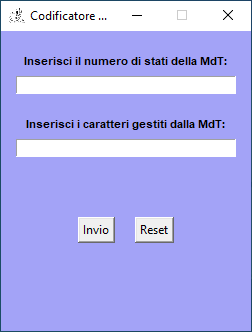
\includegraphics[width=.3\textwidth]{Images/schermata_iniziale.png}
	\caption{Schermata Iniziale}
	\label{fig:schermata_iniziale}
\end{figure}

Nella figura \ref{fig:schermata_iniziale} sono presenti due \foreignlanguage{english}{form} in cui inserire l'input; in particolar modo, nel primo \foreignlanguage{english}{form} è necessario inserire il numero di stati della macchina di Turing che si vuole simulare (è necessario inserire un numero intero maggiore di 0); nel secondo form devono essere inseriti i caratteri che vengono letti dalla macchina di Turing che si vuole simulare, i caratteri devono appartenere all'alfabeto internazionale, devono essere separati dal carattere "\emph{-}", devono essere minuscoli e non ci devono essere errori. Se almeno uno di questi vincoli viene violato, apparirà la seguente schermata di errore:

\clearpage

 \begin{figure}[h!]
	\centering
	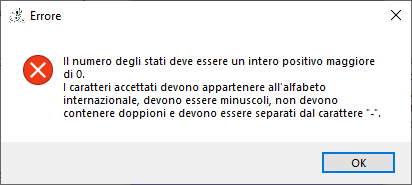
\includegraphics[width=.5\textwidth]{Images/errore_schermata_iniziale.png}
	\caption{Errore Schermata Iniziale}
	\label{fig:errore_schermata_iniziale}
\end{figure}


Nella schermata presente nella figura \ref{fig:schermata_iniziale} sono presenti oltre i due \foreignlanguage{english}{form} anche due bottoni; il bottone \foreignlanguage{english}{reset} permette di eliminare il testo inserito in precedenza nei due 	\foreignlanguage{english}{form}; una volta riempiti i \foreignlanguage{english}{form} correttamente, il bottone \emph{invio} permette di passare alla seguente schermata:

\begin{figure}[!htpb]
	\centering
	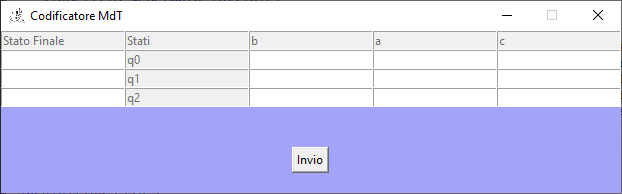
\includegraphics[width=.8\textwidth]{Images/schermata_intermedia.png}
	\caption{Schermata intermedia}
	\label{fig:schermata_intermedia}
\end{figure}

Nella schermata presente nella figura \ref{fig:schermata_intermedia} è presente una tabella di transizione in cui è possibile descrivere la macchina di Turing $M$. Inoltre, lo stato $q_0$ è sempre stato iniziale. La prima colonna della tabella è utilizzata per indicare gli stati finali della macchina di Turing; se un determinato stato, è uno stato finale allora utilizzeremo un \emph{1} altrimenti useremo uno \emph{0}; per esempio, per indicare che lo stato $q_1$ è stato finale nella cella alla sua sinistra inseriremo un \emph{1}.\\
Nella tabella vengono indicati i caratteri in cima e gli stati al lato; è necessario, pertanto, indicare per ogni cella in cui si incrocia uno stato e un carattere la relativa transizione che avviene leggendo quel determinato carattere in quel determinato stato. Per indicare la transizione è necessario indicare prima lo stato seguito dal carattere che viene scritto e il movimento della testina (è necessario inserire "\emph{l}" per indicare che la testina si sposta di una cella a sinistra o "\emph{r}" per indicare che la testina si sposta a destra); tutti questi elementi devono essere separati dal simbolo "\emph{-}". Per indicare che non avviene nessuna transizione è necessario inserire il simbolo "\emph{/}".\\
Dopo aver riempito tutte le caselle della tabella, è possibile premere il tasto "\emph{invio}", se qualche errore è stato commesso, apparirà la seguente schermata di errore:

\clearpage

\begin{figure}[!h]
	\centering
	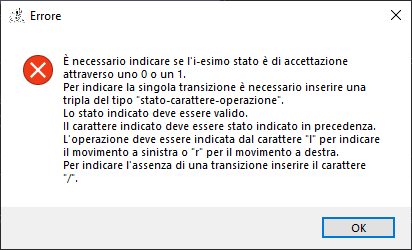
\includegraphics[width=.5\textwidth]{Images/errore_schermata_intermedia.png}
	\caption{Errore Schermata intermedia}
	\label{fig:errore_schermata_intermedia}
\end{figure}

Se invece, tutto è stato inserito correttamente, dopo la schermata di invio apparirà la seguente finestra:

\begin{figure}[!htpb]
	\centering
	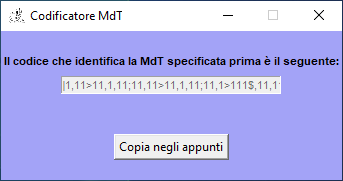
\includegraphics[width=.5\textwidth]{Images/schermata_finale.png}
	\caption{Schermata finale}
	\label{fig:schermata_finale}
\end{figure}

Una volta arrivati alla finestra rappresentata in figura \ref{fig:schermata_finale} è necessario cliccare sul pulsante "\emph{copia negli appunti}" in modo da copiare la stringa che identifica la macchina di Turing inserita; questa stringa sarà necessaria quando utilizzeremo la macchina di Turing universale.

		\section{Creazione della Stringa che Indica una MdT}

La stringa che indica una macchina di Turing $M$ contiene diversi simboli che indicano le transizioni eseguite da $M$.\\
Gli stati della macchina di Turing $M$ sono codificati in alfabeto unario utilizzando il simbolo "$1$", per esempio: indicheremo con la stringa "$1$" lo stato $q_0$, con la stringa "$11$" lo stato $q_1$, con la stringa "$111$" lo stato $q_2$ e così via; il discorso è analogo per l'alfabeto di input della macchina di Turing $M$, infatti, anche questo è codificato in alfabeto unario utilizzando il simbolo $1$, per esempio: indicheremo con la stringa "$1$" il carattere $a$, con la stringa "$11$" il carattere $b$, con la stringa "$111$" il carattere $c$ e così via.
Per le codificare le operazioni fatta dalla testina a fine computazione, viene utilizzata la stringa "$1$" per indicare il movimento della testina a sinistra e la stringa "$11$" per indicare il movimento della testina a destra.
Altri caratteri che vengono usati sono:

\begin{itemize}
	\item Il carattere "|" viene usato per indicare l'inizio delle transizioni (è sempre il primo carattere della stringa);
	\item Il carattere "\emph{,}" viene usato per separare i singoli elementi della transizione;
	\item Il carattere ">" viene usato per separare la prima parte della computazione (quando si legge un carattere dal nastro in un certo stato) con la seconda parte della computazione (in cui un carattere viene scritto sul nastro, avviene un movimento della testina e avviene il cambio di stato);
	\item Il carattere "\emph{;}" viene usato per separare le transizione;
	\item Il carattere "\emph{\$}" viene usato per indicare che un determinato stato è anche stato finale.
\end{itemize}

			\subsection{Esempio di Stringa}
			
Prendiamo per esempio questa stringa che descrive una macchina di Turing:

\begin{center}
	$|1,1>11,1,11;11,11>111\$,11,11;11,1>11,1,11;$
\end{center}

Adesso analizzeremo le singole transizioni che sono separate dal simbolo "\emph{;}":

\begin{enumerate}
	\item La transizione $1,1>11,1,11$ indica che partendo dallo stato $q_0$ e leggendo il carattere $a$, la computazione prevede che si scriva il carattere $a$, ci si sposti con la testina a destra e si arrivi allo stato $q_1$;
	\item La transizione $11,11>111\$,11,11$ indica che partendo dallo stato $q_1$ e leggendo il carattere $b$, la computazione preveda che si scriva il carattere $b$, ci si sposti a destra con la testina e si arrivi allo stato finale $q_2$; 
	\item La transizione $11,1>11,1,11$ indica che partendo dallo stato $q_1$ e leggendo il carattere $a$, la computazione preveda che si scriva il carattere $a$, ci si sposti a destra con la testina e si arrivi allo stato $q_1$.
\end{enumerate}

	\chapter{Macchina Di Turing Universale} \label{Capitolo 4}

		\section{Come Inserire L'Input}
		
La Macchina di Turing universale $M$ dispone di 3 nastri usati per la computazione, in particolar modo:

\begin{itemize}
	\item Il primo nastro è usato per contenere la stringa che indica la funzione di transizione della macchina di Turing $M'$ che si vuole simulare;
	\item Il secondo nastro contiene l'input che si vuole dare alla macchina di Turing $M'$ che si vuole simulare;
	\item Il terzo nastro è usato come "nastro di lavoro" e avrà il compito di contenere lo stato corrente e il carattere che si è letto; il terzo nastro è anche usato per aggiornare l'input ricevuto per $M'$.
\end{itemize}

L'input che si vuole inserire per la macchina di Turing $M'$ deve essere formato in questo modo:

\begin{enumerate}
	\item L'input deve appartenere all'alfabeto binario (quindi deve contenere solo $0$ e $1$);
	\item Visto che la macchina di Turing universale legge caratteri dell'alfabeto internazionale, ogni lettera è stata codificata in alfabeto unario, quindi al carattere "$a$" corrisponde la stringa "$1$", al carattere "$b$" corrisponde la stringa "$11$", al carattere "$c$" corrisponde la stringa "$111$" e così via;
	\item Ogni carattere deve essere separato dagli altri caratteri dal simbolo "$0$";
	\item Il carattere $\Diamond$ di $M$ deve essere rappresentato con un carattere dell'alfabeto internazionale codificato in alfabeto unario;
	\item La stringa deve sempre terminare con uno "$0$".
\end{enumerate}

Per esempio la stringa "$abc$" viene identificata dalla stringa "$101101110$", la stringa "$aaab$" viene identificata dalla stringa "$101010110$".\\
Quindi, per ricapitolare, nel primo nastro si deve incollare la stringa che viene restituita dal programma che è stato trattato nel capitolo \ref{Capitolo 3}, nel secondo nastro deve essere inserita  una stringa appartenente all'alfabeto binario (contenente solo $0$ e $1$) e il terzo nastro deve essere lasciato vuoto.

		\section{Spiegazione Macchina Di Turing Universale}
		
La macchina di Turing universale $M$ è costituita da numerosi stati:

\begin{itemize}
	\item $q_0$, $q_1$, $q_2$ e $q_{16}$: come detto in precedenza, lo stato iniziale di $M$ è $q_0$. Questi 4 stati hanno il compito di inizializzare il terzo nastro in modo da permettere la computazione della stringa di input. In particolar modo, questi stati permettono al terzo nastro di posizionarsi nello stato $q_0'$ della macchina di Turing $M'$ che si vuole simulare, permettendo di leggere il primo carattere dell'input e di posizionarsi nuovamente all'inizio della stringa presente sul secondo nastro;
	\item $q_3$, $q_{12}$: questi due stati sono fondamentali per iniziare la computazione. Infatti, lo stato $q_3$ ha il compito di riportare il primo nastro contenente le computazioni al simbolo iniziale (in modo da leggere tutte le computazioni), dello stato; dallo stato $q_3$ si può passare allo stato $q_{12}$, che permette di riposizionarsi al primo elemento del terzo nastro (in modo da leggere correttamente lo stato in cui ci si trova e il carattere che è stato letto);
	\item $q_4$, $q_{13}, q_{14}$: dallo stato $q_3$ si avanza allo stato $q_4$ quando sia il primo nastro che il terzo nastro si ritrovano al primo carattere; questo viene fatto per controllare se la computazione presente nel terzo nastro è possibile nelle computazioni di $M'$ indicate nel primo nastro; se le computazioni non corrispondono, lo stato $q_{13}$ riporta il terzo nastro al punto di partenza, mentre, lo stato $q_{14}$ porta il primo nastro alla prossima computazione da confrontare. Questo ciclo continua fintantoché non viene trovata una computazione compatibile (e in quel caso si passa allo stato $q_5$ andando ad aggiornare lo stato di $M$) oppure fino a quando non terminano le computazioni disponibili (in quel caso la computazione è illegale ed $M$ si ferma);
	\item $q_5$, $q_6$, $q_7$: una volta arrivati allo stato $q_5$ significa che esiste una transizione legale in $M'$, pertanto si procede con il resto della computazione; lo stato $q_5$ ha il compito di rimuovere tutto ciò che è contenuto nel terzo nastro di $M$ in modo da prepararsi per il cambio di stato; gli stati $q_6$ e $q_7$ hanno il compito di ricopiare il nuovo stato nel terzo nastro;
	\item $q_8, q_{15}, q_{17}, q_{32}, q_{18}, q_{19}, q_{23}, q_{30}, q_{31}, q_{33}, q_{34}, q_{35}, q_9$: tutti questi stati hanno il compito di aggiornare il secondo nastro (che contiene l'input) andando a revisionare il valore della cella indicata nella computazione. Per fare ciò inizialmente il contenuto del secondo nastro viene conservato a partire dal carattere successivo a quello che deve essere modificato; dopodiché, viene inserito il carattere modificato nel secondo nastro e viene copiato ciò che prima era presente dopo il carattere che è stato modificato; infine, vengono riposizionati i caratteri che sono a sinistra del carattere modificato in modo da avere una sequenza di caratteri. Al fine di questa operazione, si ritorna allo stato $q_8$ e da questo si passa a $q_9$;
	\item $q_{10}, q_{26}, q_{27}, q_{28}$: questi stati servono per simulare il movimento della testina che va a sinistra, in particolar modo, in questo caso si opera sul nastro due e si va a sinistra fintantoché non trova uno $0$; una volta trovato uno $0$, questo continua ad andare a sinistra fintantoché non trova un altro $0$. Una volta trovato si sposta di una posizione a destra (e si posiziona al primo carattere della stringa);
	\item $q_{11}, q_{20}, q_{21}, q_{22}, q_{36}, q_{24}$: questi stati servono per simulare il movimento della testina che va a destra, la situazione è analoga a quanto spiegato nel punto precedente;
	\item $q_{25}$: dopo aver simulato il movimento della testina, la computazione ricomincia a partire da $q_3$. Se nel terzo nastro è presente il simbolo "$\$$" significa che siamo giunti in uno stato finale e quindi la computazione termina.
\end{itemize}
		
	\chapter{Esempi Simulazione}
	
In seguito verranno trattati alcuni esempi per mostrare il funzionamento della macchina di Turing universale mostrata in precedenza nel capitolo \ref{Capitolo 4} e costruita in \emph{JFLAP 8.0 Beta}.

		\section{Esempio 1}
		
Nell'esempio 1 vedremo che la macchina di Turing universale, data una stringa $w$ può determinare se $w$ appartiene al linguaggio:

\begin{center}
	$L = \{a^n b | n > 0\}$
\end{center}

Il linguaggio $L$ è riconosciuto dalla seguente macchina di Turing:

\begin{figure}[!ht]
	\centering
	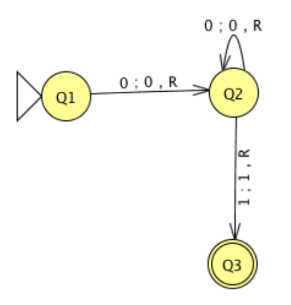
\includegraphics[width=.4\textwidth]{Images/mdt_linguaggio_1.png}
	\caption{Macchina Di Turing che riconosce $L = \{a^n b | n > 0\}$}
	\label{fig:mdt_linguaggio_1}
\end{figure}

La macchina di Turing mostrata nella figura \ref{fig:mdt_linguaggio_1} è rappresentata nel programma discusso nel capitolo\ref{Capitolo 3} nel seguente modo:

\begin{figure}[!ht]
	\centering
	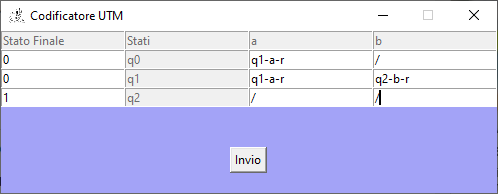
\includegraphics[width=.8\textwidth]{Images/mdt_linguaggio_1_programma.png}
	\caption{Rappresentazione della Macchina di Turing all'interno del programma}
	\label{fig:mdt_linguaggio_1_programma}
\end{figure}

La stringa che si ottiene è la seguente:

\begin{center}
	$|1,1>11,1,11;11,1>11,1,11;11,11>111\$,11,11;$
\end{center}

Possiamo testare una serie di stringhe:

\begin{itemize}
	\item La stringa "$w = aab$" viene tradotta in alfabeto binario con $1010110$, naturalmente $w \in L$, pertanto se la testiamo in $M$ otteniamo messaggio che la stringa $w$ è stata accettata;

	\begin{figure}[!ht]
		\centering
		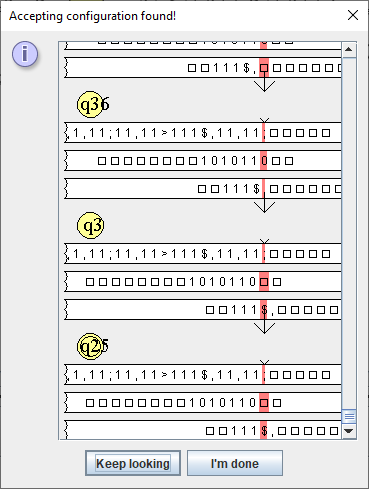
\includegraphics[width=.3\textwidth]{Images/test_1_linguaggio_1.png}
		\caption{Messaggio stringa accettata per $w = aab$}
		\label{fig:test_1_linguaggio_1}
	\end{figure}	
	
	\item La stringa "$w = baa$" viene tradotta in alfabeto binario con $1101010$, naturalmente $w \not\in L$, pertanto se la testiamo in $M$ otteniamo il messaggio che la stringa $w$ è stata rigettata.
	
	\begin{figure}[!ht]
		\centering
		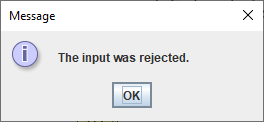
\includegraphics[width=.4\textwidth]{Images/test_errore_linguaggio.png}
		\caption{Messaggio stringa rifiutata per $w = baa$}
		\label{fig:test_2_errore_linguaggio_1}
	\end{figure}	
	
\end{itemize}	
		
		\section{Esempio 2}

Nell'esempio 2 vedremo che la macchina di Turing universale, data una stringa $w$, è in grado di determinare se $w$ appartiene al linguaggio:

\begin{center}
	$L = \{a^n b^n | n > 0\}$
\end{center}

Il linguaggio $L$ è riconosciuto dalla seguente macchina di Turing:

\begin{figure}[!ht]
	\centering
	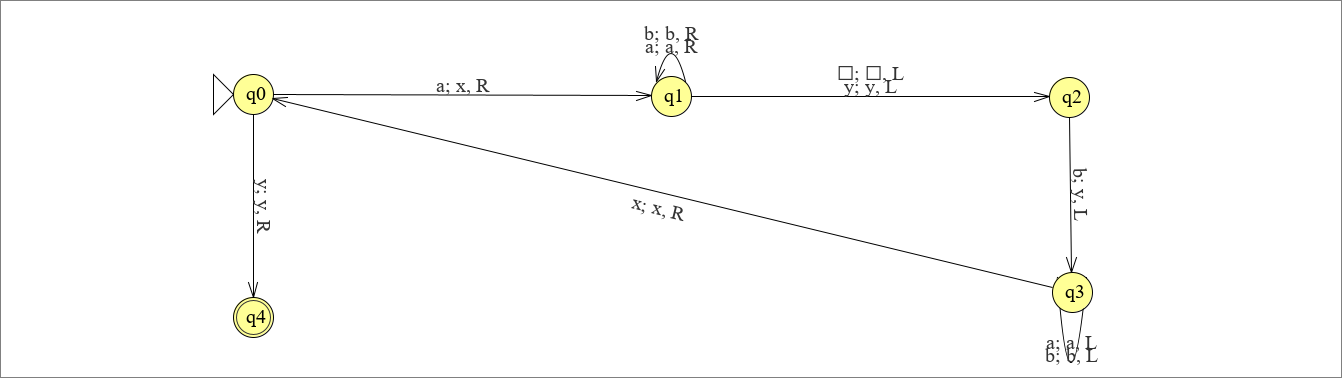
\includegraphics[width=.8\textwidth]{Images/mdt_linguaggio_2.png}
	\caption{Macchina Di Turing che riconosce $L = \{a^n b^n | n > 0\}$}
	\label{fig:mdt_linguaggio_2}
\end{figure}

La macchina di Turing mostrata nella figura \ref{fig:mdt_linguaggio_2} è rappresentata nel programma discusso nel capitolo\ref{Capitolo 3} nel seguente modo:

\begin{figure}[!ht]
	\centering
	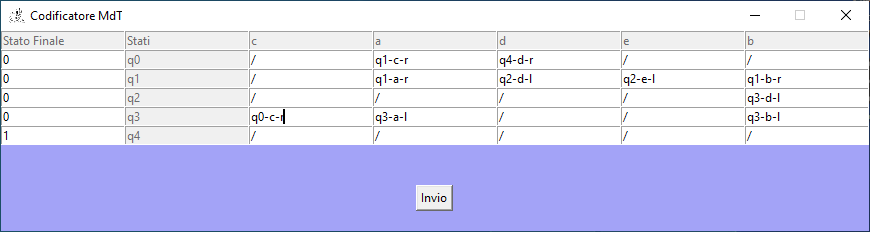
\includegraphics[width=.8\textwidth]{Images/mdt_linguaggio_2_programma.png}
	\caption{Rappresentazione della Macchina di Turing all'interno del programma}
	\label{fig:mdt_linguaggio_2_programma}
\end{figure}

La stringa che si ottiene è la seguente:

\begin{center}
	$|1,1>11,111,11;1,1111>11111\$,1111,11;11,1>11,1,11;11,1111>111,1111,1;11,11111>111,11111,1;11,11>11,11,11;111,11>1111,1111,1;1111,111>1,111,11;1111,1>1111,1,1;1111,11>1111,11,1;$
\end{center}

Possiamo testare una serie di stringhe:

\begin{itemize}
	\item La stringa "$w = aaabbb$" viene tradotta in alfabeto binario con \\$101010110110110111110$, naturalmente $w \in L$, pertanto se la testiamo in $M$ otteniamo messaggio che la stringa $w$ è stata accettata;
	
			\begin{figure}[!ht]
				\centering
				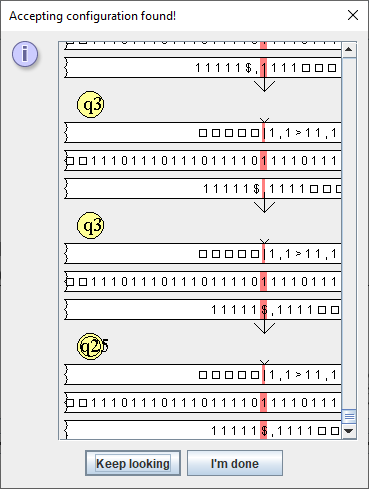
\includegraphics[width=.4\textwidth]{Images/test_1_linguaggio_2.png}
				\caption{Messaggio stringa accettata per $w = aaabbb$}
				\label{fig:test_1_linguaggio_2}
			\end{figure}
	
	\item La stringa "$w = abb$" viene tradotta in alfabeto binario con $10110110111110$, naturalmente $w \not\in L$, pertanto se la testiamo in $M$ otteniamo il messaggio che la stringa $w$ è stata rigettata.
	
		\begin{figure}[!ht]
			\centering
			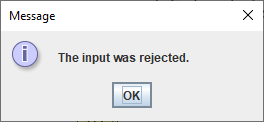
\includegraphics[width=.4\textwidth]{Images/test_errore_linguaggio.png}
			\caption{Messaggio stringa rifiutata per $w = abb$}
			\label{fig:test_2_errore_linguaggio_2}
		\end{figure}
		
\end{itemize}

\end{document}